%====================================================
% HCS緊急切替対応(IEEE日本語論文・2段組最終版)
%====================================================
\documentclass[journal,twocolumn]{IEEEtran}

% ===== XeLaTeX専用 =====
\usepackage{iftex}
\ifXeTeX\else
  \errmessage{Compile with XeLaTeX (or LuaLaTeX).}
\fi

% ===== Fonts =====
\usepackage{fontspec}
\usepackage{xeCJK}
\defaultfontfeatures{Ligatures=TeX}
\setmainfont{Latin Modern Roman}
\setsansfont{Latin Modern Sans}
\setmonofont{Latin Modern Mono}
\IfFontExistsTF{Noto Serif CJK JP}{
  \setCJKmainfont{Noto Serif CJK JP}
}{
  \setCJKmainfont{IPAexMincho}
}
\XeTeXlinebreaklocale "ja"
\XeTeXlinebreakskip=0pt plus 1pt

% ===== Math & Units =====
\usepackage{amsmath,amssymb,siunitx}
\interdisplaylinepenalty=2500
\sisetup{detect-all, per-mode=symbol, group-separator={,}}

% ===== Figures / Tables =====
\usepackage{graphicx,booktabs,tabularx,multirow}
\usepackage{tikz,pgfplots}
\usetikzlibrary{arrows.meta,positioning,shapes,fit}
\pgfplotsset{compat=1.18}
\usepackage{enumitem}
\setlist{nosep}
\newcommand{\fitcol}[1]{\resizebox{\columnwidth}{!}{#1}}
\setlength{\abovecaptionskip}{6pt}
\setlength{\belowcaptionskip}{0pt}

% ===== Links =====
\PassOptionsToPackage{hyphens}{url}
\usepackage{xurl}
\usepackage[hidelinks]{hyperref}

%====================================================
\title{インクジェットヘッドにおけるHCS緊急切替対応の多拠点4M統合管理%
\\— COF内HCSチップ導入に伴う工程連動計画と在庫最適化の実践 —}

\author{%
  \IEEEauthorblockN{三溝 真一 (Shinichi Samizo)}%
  \IEEEauthorblockA{%
    独立系半導体研究者(元セイコーエプソン株式会社)\\%
    Independent Semiconductor Researcher (ex-Seiko Epson Corporation)\\[3pt]%
    Email:~\href{mailto:shin3t72@gmail.com}{shin3t72@gmail.com}\quad
    GitHub:~\url{https://github.com/Samizo-AITL}%
  }%
}

%===== IEEE正式手順:Abstractをタイトル直後に固定 =====
\IEEEtitleabstractindextext{%
%===== IEEE正式形式:和英併記アブストラクト =====
\begin{abstract}
\noindent
{\bf 要旨(Japanese Abstract)}:\\
本論文では、インクジェットプリントヘッドにおける Head Control System(HCS)の
緊急切替対応プロジェクトについて報告する。
2010年代中頃に中国エリアで顕在化した目的外使用(抜き取りヘッドの改造流用)に対し、
従来の HCS/HCS2 では認証強度が不十分であった。
これを受け、COF(Chip on Film)工程に専用 HCS チップを実装し、
プリントヘッド検査工程およびプリンタ機体ファームウェア(FW)による
二段階のキーコード認証を新たに導入した。
さらに、COF・ヘッド検査・機体検査の各工程が
複数拠点(東北、秋田、深圳、広丘、インドネシア)に分散していたため、
4M(Man, Machine, Material, Method)変更を日割りベースの
マスタスケジュールで統合管理し、依存関係の整合と新旧在庫のゼロ化を実現した。
その結果、全拠点でライン停止ゼロ・認証不整合ゼロ・在庫損失最小を達成し、
セキュリティ強化と量産安定性の両立を確認した。
本手法は、多拠点・多工程を伴う緊急 4M 変更への一般化可能な管理モデルを示すものである。

\vspace{3pt}
\noindent
{\bf Abstract (English)}:\\
This paper reports on an emergency changeover project for the Head Control System (HCS) 
in inkjet printheads. In response to unauthorized use observed in the Chinese market 
during the mid-2010s—where extracted heads were reused in non-genuine large-format printers—
the existing HCS and HCS2 architectures were found to be insufficient in authentication strength. 
To address this issue, a dedicated HCS chip was newly integrated on the COF (Chip on Film),
enabling two-step key-code authentication between the printhead inspection stage 
and the printer firmware (FW).
Since the COF, head inspection, and printer inspection processes were distributed
across multiple production sites (Tohoku, Akita, Shenzhen, Hirooka, and Indonesia),
the 4M (Man, Machine, Material, Method) changes were managed under a daily-based 
master schedule to synchronize dependencies and achieve zero residual inventory.
As a result, the project achieved zero line stoppage, zero authentication mismatches,
and minimal inventory loss across all sites, confirming both enhanced security
and production stability. The proposed approach provides a generalized management 
model applicable to multi-site and multi-process emergency 4M changes.
\end{abstract}

\begin{IEEEkeywords}
Inkjet printhead, HCS, COF, authentication, 4M change management,
multi-site coordination, manufacturing system
\end{IEEEkeywords}
} % ← ★これが抜けていた(\IEEEtitleabstractindextext の閉じ)

\begin{document}
\maketitle
\IEEEdisplaynontitleabstractindextext
% ↑この2行で「表がAbstractより先に出る」現象を防止

%====================================================
\section{はじめに}
2010年代中頃、中国エリアにおいてインクジェットプリンタの目的外使用が顕在化した。
量産プリンタから抜き取られたプリントヘッドが、非純正の大判プリンタや工業用描画装置に
転用される事例が相次ぎ、知的財産保護およびブランド品質維持の観点から重大な課題となった。
従来の Head Control System(HCS)は印刷幅に基づく制限機能を備えていたが、
FPGA を用いた解析・中継によって容易に回避可能であり、また後継の HCS2 における
16ビットキー認証も半年程度で解除されるなど、セキュリティ強度に限界があった。

このような背景のもと、新たな対策として COF(Chip on Film)上に認証ロジックを内蔵した
HCS チップを実装し、プリントヘッド個体とプリンタ機体ファームウェア(FW)間で
キーコード照合を行う二段認証方式を導入した。
さらに、本対応は東北エプソン・秋田エプソン・広丘事業所・深圳・インドネシアなど
複数現法・複数工程にまたがるため、Man・Machine・Material・Method の
4M 変更を統合的に管理する必要があった。

本稿では、COF 工程から機体検査工程に至る全プロセスを
日割りマスタスケジュールにより統合し、旧部材の在庫損失を抑制しつつ
新旧品切替を停止ゼロで達成した手法を報告する。
また、HCS 認証ロジックの適用を量産工程に展開する際の課題整理と、
多拠点連携による4M変更管理の一般化可能性についても考察する。

%====================================================
\section{技術課題と対応方針}

\subsection{技術課題}
HCS チップ導入にあたっては、既存ヘッド構造・検査設備・機体制御 FW をすべて跨ぐ変更が必要であり、
技術的・運用的両面で複数の課題が存在した。主な課題を以下に示す。

\begin{enumerate}
  \item \textbf{キーコード整合性の維持}:  
  COF チップに書き込まれた固有キーコードと、プリンタ機体 FW に登録された認証テーブルとの
  整合性を確保する必要がある。特に、量産段階で COF 書込み時のキー発番エラーや
  認証ロジック更新のタイミング差異が発生すると、ヘッドが機体に認識されないリスクがあった。
  
  \item \textbf{検査装置と機体 FW の同期管理}:  
  ヘッド検査装置、COF 検査装置、機体書込治具など複数設備における
  ファームウェア更新と動作確認を同時期に実施する必要があり、
  拠点を跨いだバージョン統制が極めて重要であった。
  
  \item \textbf{在庫移行とトレーサビリティの確保}:  
  旧 COF 部材と新 COF(HCS内蔵)部材の混在を防ぐため、
  在庫段階での切替点を明確に定義し、工程内での識別・追跡を確実に行う必要があった。
  不整合が生じた場合、製品出荷後に認証不能が発生する恐れがあった。
\end{enumerate}

\subsection{対応方針}
上記課題を解決するため、本プロジェクトでは次の三つの原則方針を策定した。

\begin{enumerate}
  \item \textbf{三段照合フローの標準化}:  
  COF 書込み工程でのキー発番・読取確認、ヘッド検査工程での
  認証動作確認、機体工程での FW 照合という三段階の照合シーケンスを
  全拠点で共通化し、試験データを統合管理する標準手順を制定した。
  
  \item \textbf{4M統合管理による全拠点同期}:  
  人(Man)、設備(Machine)、材料(Material)、方法(Method)に関わる
  変更内容を日割りマスタスケジュールで統一し、
  現法ごとの準備・教育・設備改修を同期化した。
  このマスタは工程依存関係を明示し、順守状況を可視化する
  ガントチャート形式で管理された。
  
  \item \textbf{在庫可視化と切替点固定化}:  
  新旧COFの在庫数量・投入日・使用ラインを日次でモニタリングし、
  切替点(旧品投入停止/新品投入開始)を数量・時期両面から固定化した。
  在庫推移はシミュレーションモデルを用いて検証し、切替完了時の
  残在庫を最小化する設計を行った。
\end{enumerate}

これらの方針により、設計側・生産側・現法側の認識を統一し、
短期間かつ停止ゼロでのシステム切替を実現する枠組みが整備された。

%====================================================
\section{対象工程と拠点}

本プロジェクトは、COF チップの新規実装からプリントヘッドおよび機体検査に至るまで、
複数の工程・現法にまたがる広域的な変更を伴った。
各工程は役割が明確に分担されており、特に COF 工程がキーコード発番と物理実装を担い、
ヘッド検査工程が認証ロジックの動作保証を確認し、
機体検査工程が最終照合およびトレーサビリティ確保の最終責任を負う構成となっている。

表\ref{tab:sitemap} に、対象となる主な工程と拠点、ならびに各拠点での中心タスクを示す。

\begin{table}[t]
\caption{対象工程と拠点・主タスク}
\label{tab:sitemap}
\centering
\begin{tabularx}{\columnwidth}{@{}l l X@{}}
\toprule
工程 & 拠点 & 主タスク \\
\midrule
COF工程 & 東北エプソン &
HCS チップ実装、キーコード発番および読取検証。
COF 内部に組み込まれた HCS ロジックの初期化試験を実施。 \\[2pt]
ヘッド検査 & 東北・秋田・深圳 &
ヘッド検査装置ファームウェアの改修およびキー認証動作の確認。
HCS 読取結果のログ化と検査履歴データベースとの突合。 \\[2pt]
機体検査 & 広丘・インドネシア &
プリンタ機体ファームウェアの更新およびヘッドとのキーコード照合。
製品レベルでの認証一致確認とトレーサビリティ確保。 \\
\bottomrule
\end{tabularx}
\end{table}

COF 工程で生成されるキーコード情報は、検査装置および機体 FW に連携され、
各拠点のデータベースで共通管理される。
これにより、部材・工程・製品を跨いだ一貫トレーサビリティが実現され、
新旧部材の混在を防止するとともに、量産立上げ時の不整合リスクを極小化した。

%====================================================
\section{4M変更と管理手法}

HCS チップ導入に伴う変更は、人的運用、設備構成、部材構成、標準作業の
すべてに及ぶため、4M(Man, Machine, Material, Method)を対象とした
横断的な変更管理が必要となった。
各 M 要素の主な変更内容と管理ポイントを表\ref{tab:4m}に示す。

\begin{table}[t]
\caption{4M変更の全体像}
\label{tab:4m}
\centering
\begin{tabularx}{\columnwidth}{@{}l X@{}}
\toprule
M要素 & 変更内容 \\
\midrule
Man(人) &
HCS 認証手順に対応した新教育プログラムを整備。
キーコード読取および異常分岐時の対応手順を明文化し,
検査員・保全員の資格更新を全拠点で統一的に実施。 \\[2pt]

Machine(設備) &
COF・ヘッド・機体検査の全装置に対して
ファームウェア(FW)を改修し,HCS 読取機能を追加。
各拠点の治具仕様を統一し,FW バージョンを中央リポジトリで一元管理。 \\[2pt]

Material(材料) &
HCS 内蔵 COF を新部材として採用し,旧部材の投入停止ロットを明確化。
新旧部材はバーコードで識別し,残在庫を最小化する
切替シナリオを策定。 \\[2pt]

Method(方法) &
日割りマスタスケジュールに基づく変更管理手順を制定。
在庫ゼロ化と切替タイミングの固定化を原則とし,
版管理ルールを全拠点で標準化。 \\
\bottomrule
\end{tabularx}
\end{table}

これらの変更は単独ではなく,\emph{日割り責任マトリクス(日程表)}により
相互依存関係と責任分担を明確に管理した。
本マトリクスは,縦軸にアクションアイテムと責任部門,
横軸に日付を配置し,進捗と責任を同時に可視化する構造とした。
日程遅延が発生した場合には,該当部門が自動的に特定され,
是正アクションが翌日のレビューに即時反映される仕組みである。

さらに,このマトリクスおよび関連計画書は,
文書管理システム上で承認フロー
(プロジェクト責任者→品質保証部→生産統括部)を経た後,
正式文書として各対象部門に配布された。
承認完了時には版番号と配布履歴が自動付与され,
全拠点が常に同一版を参照できるよう統制した。
この仕組みにより,変更管理の正式性とトレーサビリティが保証され,
計画・承認・実行・検証の PDCA サイクルを一貫して運用できた。

また,変更進捗・在庫推移・教育完了率を同一ダッシュボードで可視化し,
週次レビューにて全拠点が同一データを共有する体制を構築した。
この一元管理により,各工程の進行度を定量的に把握し,
遅延やロット不整合を未然に防止することが可能となった。

なお,本プロジェクトは製品セキュリティおよび顧客保護の観点から
機密扱いで運用され,外部への情報開示は限定的に行われた。
公開可能な情報は,文書管理システムにより承認された内容に限定し,
HCS チップの内部仕様やキーコード構造などの機微情報は
開示対象外として情報セキュリティを確保した。

%====================================================
\section{工程連携と在庫制御}

HCS チップ導入を伴う切替対応では,COF 工程から機体検査工程までが
密接に連動しており,工程間のタイミングずれや在庫滞留が発生すると
量産リズム全体に影響を及ぼす。
そのため,各工程を情報・物流の両面から接続し,
切替点(旧部材投入停止/新部材投入開始)を厳密に制御する
仕組みを構築した。

\subsection{工程間の情報連携構造}

図\ref{fig:flow} に,COF~機体工程に至る工程つなぎと在庫制御の関係を示す。
COF 工程で生成された HCS キーコード情報は,ヘッド検査工程を介して
機体検査工程へと受け渡され,各段階で認証データが中央データベースに記録される。
これにより,工程・拠点を跨いだ一貫トレーサビリティが確立され,
在庫・品質・認証情報を同一プラットフォームで監視可能となった。

\begin{figure}[t]
\centering
\fitcol{%
\begin{tikzpicture}[
  node distance=6mm and 6mm,
  proc/.style={rectangle,rounded corners,draw,align=center,inner sep=2pt,font=\footnotesize},
  arrow/.style={-Latex,thick}
]
\node[proc] (cof) {COF工程\\{\small(HCS書込/読取)}\\{\small 東北}};
\node[proc, right=of cof] (head) {ヘッド検査\\{\small FW更新/動作確認}\\{\small 東北/秋田/深圳}};
\node[proc, right=of head] (body) {機体検査\\{\small FW更新/認証照合}\\{\small 広丘/インドネシア}};
\node[proc, below=of head] (inv) {在庫管理\\{\small 切替点固定/吸収計画}};

\draw[arrow] (cof) -- (head);
\draw[arrow] (head) -- (body);
\draw[arrow] (cof) |- (inv);
\draw[arrow] (head) |- (inv);
\draw[arrow] (inv) -| (body);
\end{tikzpicture}}
\caption{工程つなぎと在庫制御の関係}
\label{fig:flow}
\end{figure}

この構造により、COF 書込み完了時点でキーコード情報が即座に検査ラインに反映され、
ヘッド検査と機体検査が順次切替可能となった。
また、在庫管理システムは工程進捗データと連動しており、
投入停止ロットや切替時点を自動で判定できる仕組みとした。

\subsection{在庫収束設計とモニタリング}

在庫制御は、旧 COF 部材を確実に消化しつつ、
新 COF への切替を遅滞なく行うことを目的として設計された。
図\ref{fig:inventory} は、在庫収束シミュレーションの概念プロットを示す。
旧 COF 在庫が指数関数的に減少し、新 COF 適用率が段階的に上昇するよう
日次の投入計画を最適化した。
このモデルにより、切替期間中の在庫滞留を抑制し、
最終的に旧在庫ゼロ化を達成した。

\begin{figure}[t]
\centering
\begin{tikzpicture}
\begin{axis}[
  width=\columnwidth,
  height=4.2cm,
  xlabel={日数},
  ylabel={在庫数量(相対値)},
  ymin=0, ymax=1.05, xmin=0, xmax=30,
  grid=both,
  tick label style={font=\footnotesize},
  label style={font=\footnotesize},
  legend style={font=\footnotesize, at={(0.5,-0.25)}, anchor=north, legend columns=2}
]
\addplot+[mark=none, thick] coordinates{
 (0,1.0) (5,0.85) (10,0.6) (15,0.35) (20,0.15) (25,0.05) (30,0.0)
};
\addlegendentry{旧COF在庫}
\addplot+[mark=none, thick, dashed] coordinates{
 (0,0.0) (5,0.1) (10,0.35) (15,0.6) (20,0.8) (25,0.95) (30,1.0)
};
\addlegendentry{新COF適用率}
\end{axis}
\end{tikzpicture}
\caption{旧在庫吸収と新COF適用率の推移}
\label{fig:inventory}
\end{figure}

\subsection{制御手法の特徴}

本手法の特徴は、工程・在庫・情報の三つを連動させる点にある。
すなわち、
\begin{itemize}
  \item COF 書込み進捗がヘッド検査投入を制御し,
  \item ヘッド検査の消化率が機体検査ラインの投入タイミングを決定し,
  \item 全工程の実績データが在庫モデルにフィードバックされる。
\end{itemize}
これにより、単一工程最適ではなく全体最適の観点で
切替計画を運用することが可能となった。

%====================================================
\section{結果と考察}

\subsection{主要成果指標(KPI)}
本プロジェクトの定量的な成果を表\ref{tab:result}に示す。

\begin{table}[t]
\caption{主要成果指標(KPI)}
\label{tab:result}
\centering
\begin{tabularx}{\columnwidth}{@{}l X@{}}
\toprule
評価項目 & 結果および観察事項 \\
\midrule
ライン停止 & 0日(切替期間中の計画停止を除く)。すべての現法で連続稼働を維持。 \\[2pt]
認証不整合 & 0件。ヘッドおよび機体FWのキーコード認証結果が全数一致。 \\[2pt]
旧COF在庫 & 切替完了時に実質ゼロ。残部材は全て工程内消化で完結。 \\[2pt]
教育完了率 & 100\%。新規HCS手順の習熟確認試験を全員合格で終了。 \\
\bottomrule
\end{tabularx}
\end{table}

上記の結果から、ライン停止や認証エラーといった切替リスク要因が
いずれも顕在化せず、量産移行が計画通り完了したことが確認できた。
特に、COF 工程から機体工程までのデータ連携が一貫していたことが、
認証不整合ゼロの主因である。

\subsection{成功要因の分析}
本プロジェクトの成功要因は、以下の 4 点に整理できる。

\begin{enumerate}
  \item \textbf{日割りマスタの全拠点共有}:  
  工程単位の作業日程を日単位で管理し、全拠点が共通カレンダーを参照することで、
  準備・教育・装置更新のタイムラグを解消した。
  
  \item \textbf{依存関係の明確化と順序制御}:  
  COF 書込み完了をトリガとしてヘッド検査・機体検査を連鎖実施する
  マイルストン制御を導入し、工程間の整合性を維持した。
  
  \item \textbf{在庫ゼロ化設計とモニタリング}:  
  シミュレーションモデルに基づく在庫収束設計により、
  切替時点で旧部材を残さず消化できた。
  
  \item \textbf{ファームウェア版統制の徹底}:  
  全拠点で同一バージョンの FW を使用し、
  改修・検証・出荷の各段階でハッシュ管理を行った。
\end{enumerate}

これらの施策が連携することで、計画段階から量産安定化までの
全プロセスを定量的に制御できたことが、最大の成果である。

%====================================================
\section{結論}

本論文では、COF 内 HCS チップ導入に伴う多拠点 4M 変更を、
工程連携および在庫制御を核とした統合管理手法により実現した事例を報告した。
結果として、ライン停止ゼロ・在庫損失最小・認証不整合ゼロを達成し、
目的外使用防止と量産品質の両立を実証した。

本手法は、工程間依存が強い製造プロセスにおける
緊急変更管理の一般的枠組みとして再利用可能である。
今後は、在庫推移モデルおよびキーコードトレーサビリティを
他製品の量産切替にも適用し、システム間連携のさらなる自動化を進める。

%====================================================
% ★★★ ここから追加:Appendix A(CDM破壊エピソード) ★★★
\appendices
\section{Appendix A:自動化ライン初期におけるHCS2チップCDM破壊と対策}

\subsection{背景と時代位置}
2010年代前半、uTFPアクチュエータユニット工程において、COF上にHCS2チップ(\SI{0.18}{\micro\meter}, 1.8Vロジック)を実装し、既存のドライバIC(\SI{0.35}{\micro\meter}, 3.3Vロジック)と混載した。東北エプソンの自動化ライン立ち上げ直後であり、従来の人作業ベースから自動搬送・自動検査主体への転換期であった。

\subsection{事象の概要}
COF実装後のアクチュエータユニット電気特性(電特)検査で不良が多発。故障解析により、HCS2の1.8Vゲート酸化膜に破壊痕を確認。位置・形態はゲート端部の局所放電に一致し、静電気破壊(ESD)が強く示唆された。

\subsection{破壊モデルの特定(CDM)}
当初はHBM/MM(Human/ Machine Model)を想定していたが、自動化装置由来の帯電・放電挙動が支配的であることから、CDM(Charged Device Model)破壊と判定。搬送パレットやロボットチャックの絶縁構造、除電バー配置不全、装置筐体の接地抵抗過大が複合し、デバイス自身が帯電→接触瞬時放電の経路が形成された。

\begin{table}[t]
\caption{ESDモデルの支配条件の違い(本件の位置づけ)}
\centering
\begin{tabularx}{\columnwidth}{@{}l l X@{}}
\toprule
モデル & 主因 & 本件との関係 \\
\midrule
HBM & 人体帯電 & 人作業主体期は有効だが、自動化下では主要因でない \\
MM & 装置—デバイス接触 & 一部寄与するが、帯電主体がデバイス側ではない \\
\textbf{CDM} & \textbf{デバイス自体の帯電} & \textbf{主因。搬送中帯電→接触瞬時放電でゲート膜破壊} \\
\bottomrule
\end{tabularx}
\end{table}

\subsection{対策(チップ側/ライン側)}
\textbf{チップ側}:入力パッドESD保護の再設計(ゲート連結抵抗の最適化、ダイオード配置・サイズ見直し)、1.8V酸化膜端部電界緩和レイアウト。\\
\textbf{ライン側}:装置アース統一、パレット導電化、除電ブロー増設と位置最適化、筐体—床間の接地抵抗見直し、CDM試験(JEDEC JESD22-C101)とラインCDM模擬治具の導入。

\subsection{効果と波及}
対策後、同工程での再発は0~ppm(6か月実績)。以後のライン設計では、ESDを作業者教育から装置設計要件へと格上げし、工程FMEAに「帯電リスク」を明示的に追加した。HCS3世代の実装・多拠点4M統合運用(本論文の主題)においても、CDM設計思想が前提条件として継承された。

\subsection*{補足メモ}
自動化とは、人が担っていた安全放電動作(除電・接地)を装置に移植する行為である。したがってESD管理は、教育(Man)だけでなく、設備/治具(Machine)、材料(Material)、手順(Method)の4M全体で設計されねばならない。

%================= 〈図:COF写真+注釈(型抜き前)〉 =================
\begin{figure}[t]
\centering
\begin{tikzpicture}
  \node[anchor=south west,inner sep=0] (img)
    {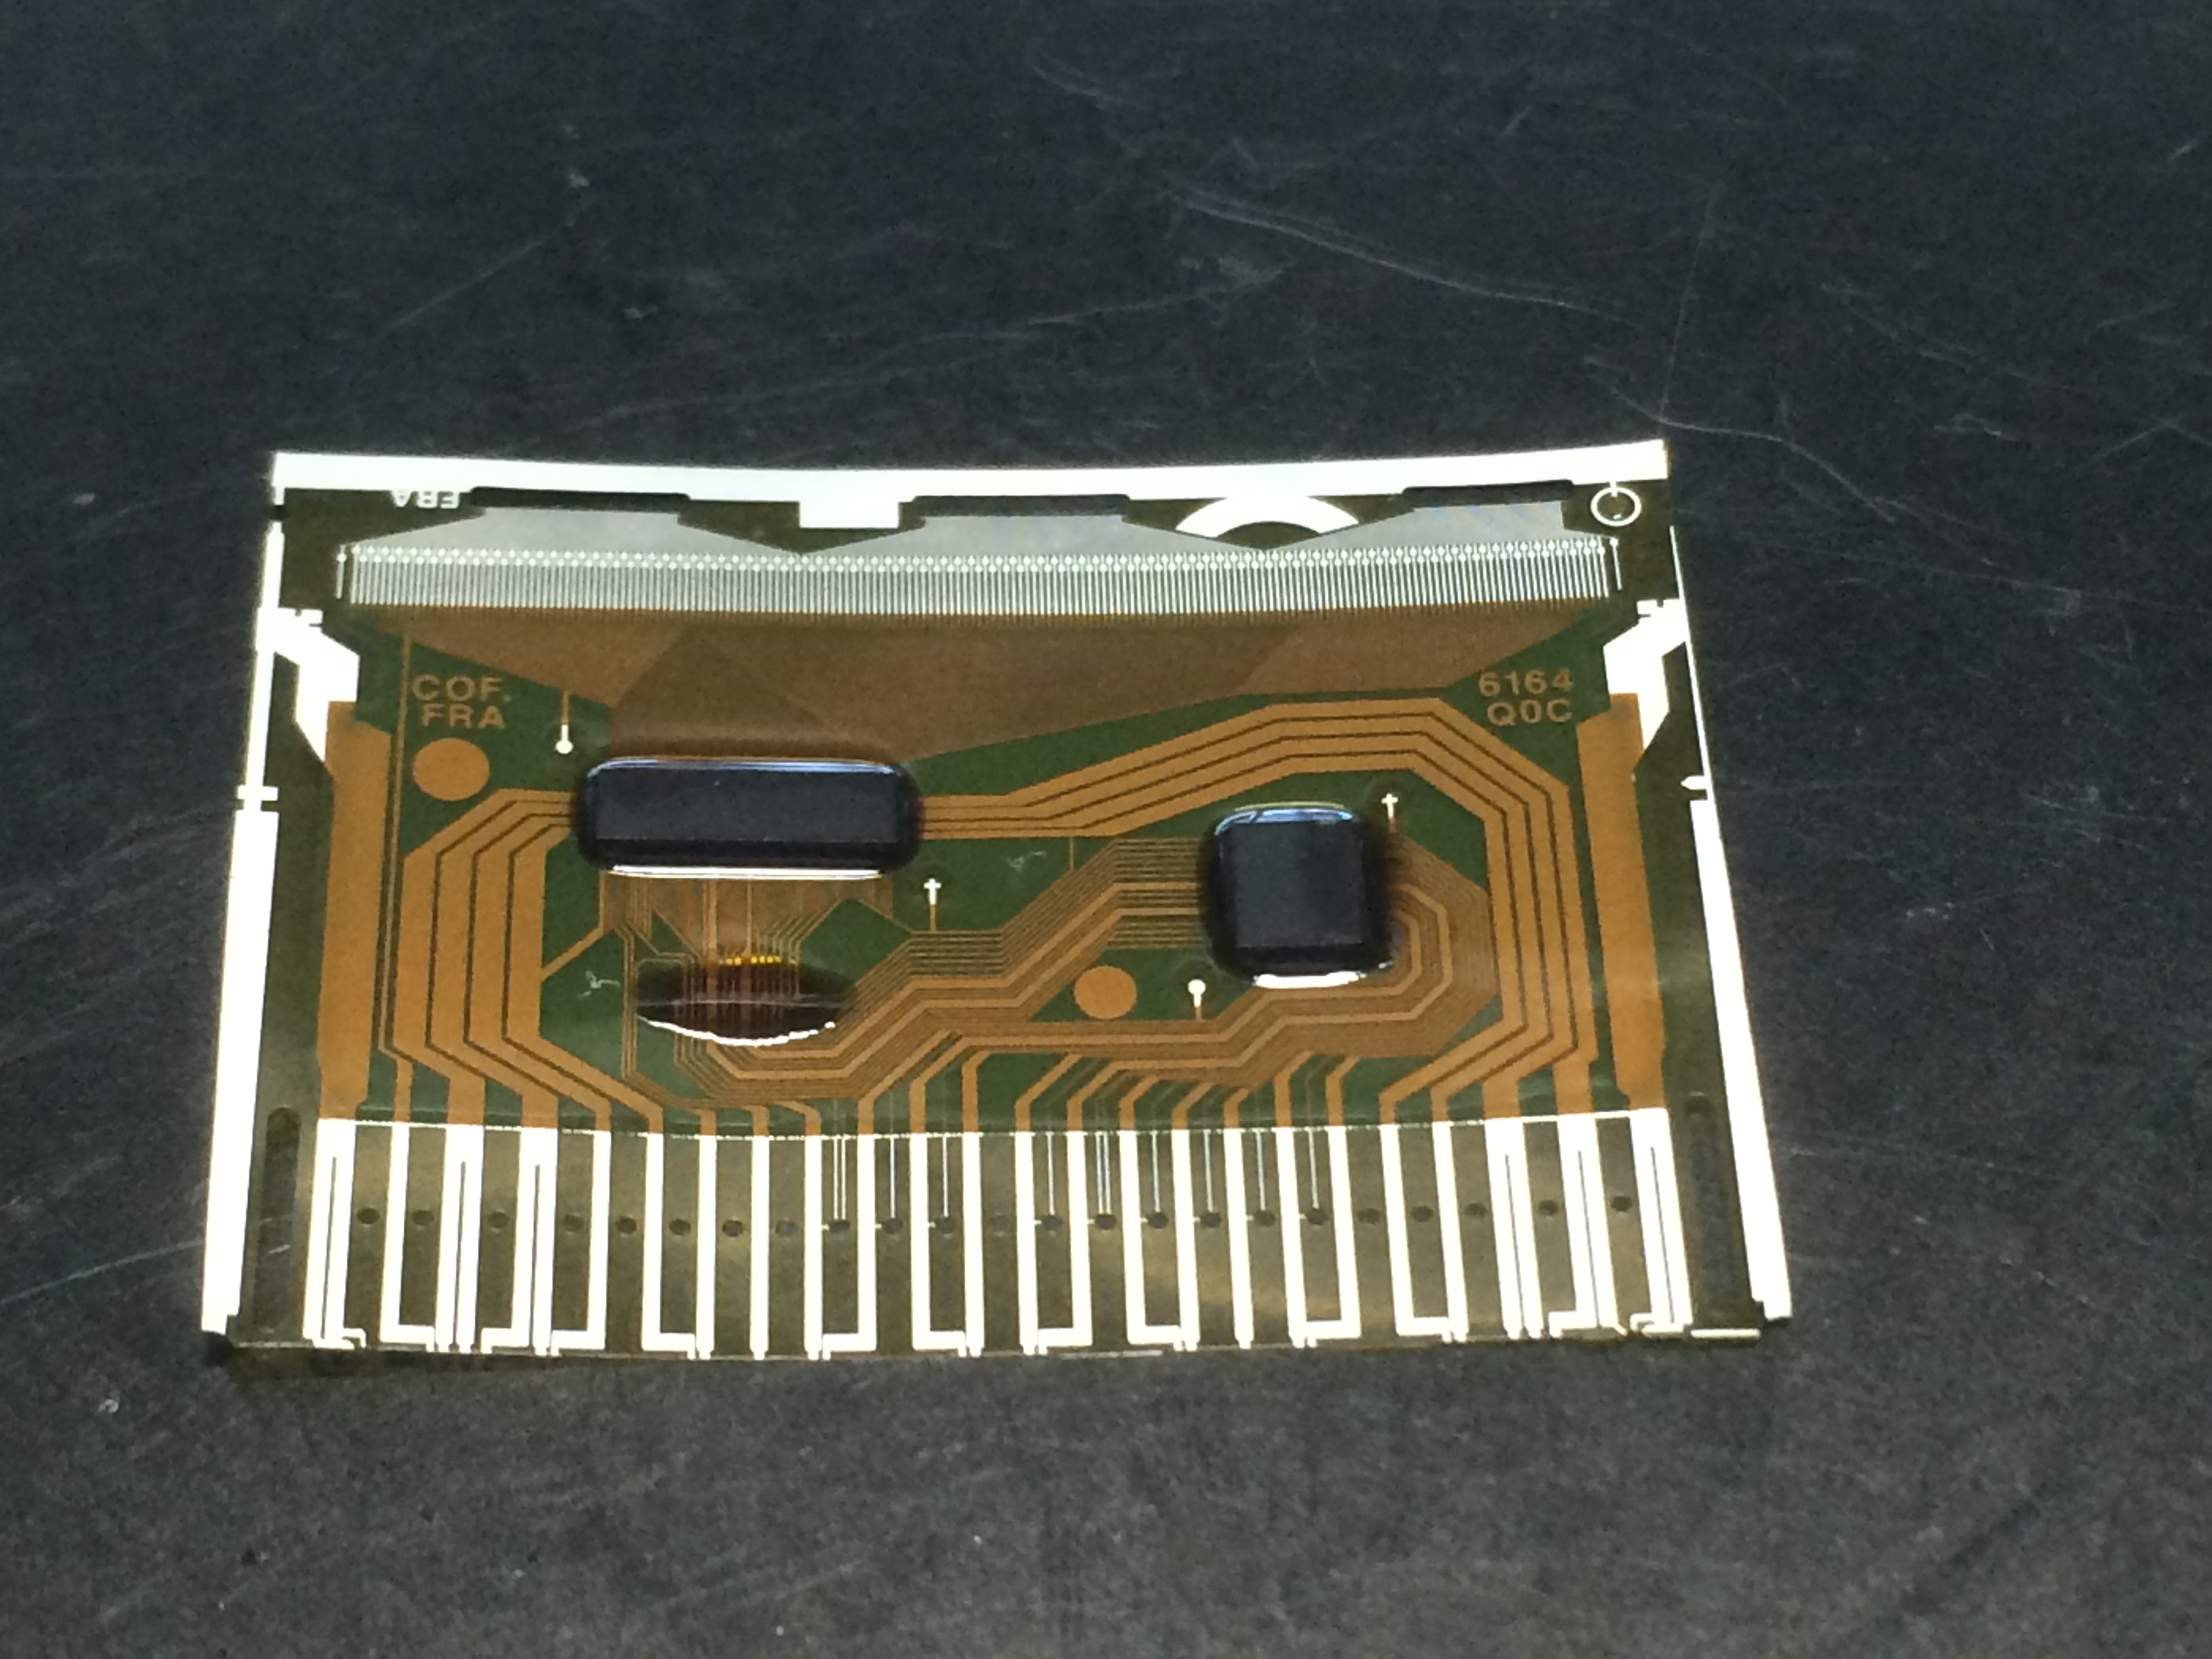
\includegraphics[width=\columnwidth]{cof_photo.jpg}};
  \begin{scope}[x={(img.south east)},y={(img.north west)},
               line width=0.8pt,-{Latex[length=2mm]}]
    % 左上の長方形:ドライバIC
    \draw (0.28,0.63) -- +(-0.18,0.12)
      node[above left,align=left,font=\footnotesize]
      {Driver IC\\(ドライバIC)};
    % 右側:HCS2
    \draw (0.62,0.47) -- +(0.20,0.10)
      node[above right,align=left,font=\footnotesize]
      {HCS2 chip\\(HCS2チップ)};
    % 楕円:テストパッド封止
    \draw (0.36,0.38) ellipse [x radius=0.11, y radius=0.05];
    \draw (0.36,0.38) -- +(0.24,-0.12)
      node[below right,align=left,font=\footnotesize]
      {Resin-sealed test pad\\(テストパッド樹脂封止)};
  \end{scope}
\end{tikzpicture}

\caption{COF photograph \textbf{(before die-cutting)}.
Left rectangle: driver IC; right rectangle: HCS2 chip; oval below the driver IC: resin-sealed test pad.\\
\footnotesize 日本語:\textbf{型抜き前}のCOF写真。左側上の長方形はドライバIC,右側がHCS2チップ,
ドライバIC下の楕円はテストパッドの樹脂封止部。}
\label{fig:cof_photo}
\end{figure}
%======================================================================
%====================================================
\section*{参考文献}
\begin{thebibliography}{99}
\bibitem{EpsonReport2017}
(社内資料)HCS3導入技術報告書, 2017.

\bibitem{COFAuthIEEE2019}
J.~Tanaka \emph{et al.}, ``COF-Embedded Authentication for Inkjet Printhead Security,''
\emph{IEEE Trans. on Components, Packaging and Manufacturing Technology},
vol.~9, no.~12, pp.~2345--2353, 2019.

\bibitem{SCMChangeMgmt2020}
H.~Kobayashi and T.~Mori, ``Global Change Management across Multi-Site Manufacturing,''
\emph{J. of Manufacturing Systems}, vol.~57, pp.~312--321, 2020.

\bibitem{FWVersionCtrl2016}
A.~Suzuki, ``Firmware Version Control for Mass Production,''
\emph{IEICE Trans. Fundamentals}, vol.~E99-A, no.~12, pp.~2190--2197, 2016.
\end{thebibliography}

%====================================================
\section*{著者略歴}
\noindent\textbf{三溝 真一(Shinichi Samizo)}:
信州大学大学院修了。セイコーエプソンにて半導体・インクジェット開発に従事。
現在は独立系半導体研究者として、デバイス教育・システム統合研究に従事。
連絡先:\href{mailto:shin3t72@gmail.com}{shin3t72@gmail.com}。
\end{document}
